\part{Migrate Excel spreadsheet dashboard to a simple REST+HTML/JS
application}
\label{c_phaseone}

\chapter*{Motivation}
\addcontentsline{toc}{chapter}{Motivation}
In order to track and follow up project's status, we built a simple tool in a
spreadsheet that linked with a database allowed us to log each change (aka
\emph{event}) on the project status on the following scope: phase change
end/start, delay, launch.

This tool also gave us a good view about different selected KPI \footnote{Key
Performance Indicator}. And based on those indicators we built few reports:
Project's events, Projects launched, Projects delayed (and detail), Projects
Gantt and Project's timelines.

The tool was fine for a while, but it took to much time to load all data
from the database, and also was not fully compatible with all users, because of
the need to install some extra required components like the ODBC for those with
Windows, or not even compatible with those using Linux computers, because the
tool was built on Microsoft Excel.

So, imagine trying to track project's \emph{events} on a tool that is slow
and not compatible with everybody. At the end we stopped using it.

Then, a fresh motivation came up to build something better,
usable for all required users and faster enough to aim the objective: track,
analyze and decide. 

The challenge was there and as well the information on the database, so it was
just a matter to migrate the spreadsheet (the view) to a HTML page with some JS,
as first client, so we decople it from any need of 3rd party component such as
ODBC, having in the middle a RESTful service that
controls the communication between the client (web browser) and what matters, the data (the model).

\chapter{Current Excel architecture}
At the beginning, the idea was to have the data centralized
\label{t_main_objective} and implement, in a fast way, a client that could show
it. The quicker solution, not always the right one but useful for a while, was
to define the simpliest database model to  track the maximum amount of events with enough value to evaluate a the
efficiency of a project and learn from our mistakes. Together with the database
we setup a Excel spreadsheet that loads the data from the defined database, but
we also needed to build different reports, so we difined few \emph{views} based
on the required KPIs, so we could query it from the external spreadsheet
without define any kind of logic, that could increase the complexity.\\

In short, elements defined are listed as follow:
\begin{itemize}
  \item A MySQL database with one table called Events used to store any possible
  event (previously defined the set of them)
  \item Few views used to achieve defined reports
  \item A Microsoft Excel spreadsheet used to show data returned by the views
  \item One connection per report used to connect Excel with the database
  via ODBC as data connectivity abstractor. 
\end{itemize}

You can see the relationship between above listed components on the 
\reffigure{f_excel_architecture}.
 
\begin{figure}[ht!]
	\centering
   	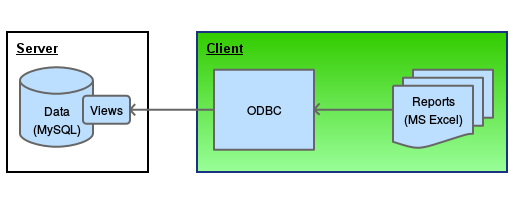
\includegraphics[width=1\textwidth]{./resources/excel_architecture.png}
   	\caption{Reports architecture using Excel}
   	\label{f_excel_architecture}
\end{figure}

\section{Database model}
Database model was defined as simple as possible, keeping in mind
possible normalization in the future without having a big impact on the data. So
decission was to use
\emph{Enum}\footnote{\url{https://dev.mysql.com/doc/refman/5.0/en/enum.html}}
data type for those fields that are static or with a predefined set of
elements like: country, project\_type or  type fields
(\reffigure{f_data_model}).

\begin{figure}[ht!]
	\centering
   	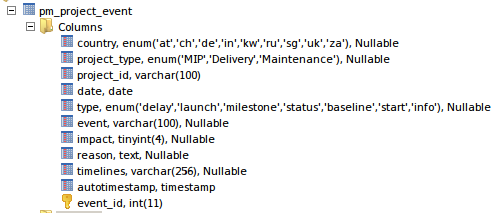
\includegraphics[width=1\textwidth]{./resources/data_model.png}
   	\caption{Data model}
   	\label{f_data_model}
\end{figure}

The most relevant field here is \emph{type}, where covers all required possible
scenarios in a project's lifetime that we needed to track. And base on that, 
reports (views) can show the specific information to be analyzed.

\section{Views definition and reports}
As described on the previous sections, we defined five reports, they are:

\begin{itemize}
  \item Amount of launches, per country and month
  \item Total project's delay
  \item Project's delays in detail
  \item Gantt chart
  \item Project's timelines chart 
\end{itemize}

On top of them, we also added an extra report listing all project's events,
just for our reference.

You can see screenshots on how they look for each of them on
\reffigure{f_report_launches}, \reffigure{f_report_delays},
\reffigure{f_report_delays_detail}, \reffigure{f_report_gantt},
\reffigure{f_report_timelines} and \reffigure{f_report_events}.

\begin{figure}[ht!]
	\centering
   	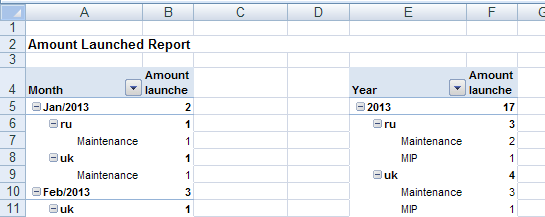
\includegraphics[width=1\textwidth]{./resources/report_launches.png}
   	\caption{Launches report}
   	\label{f_report_launches}
\end{figure}
\begin{figure}[ht!]
	\centering
   	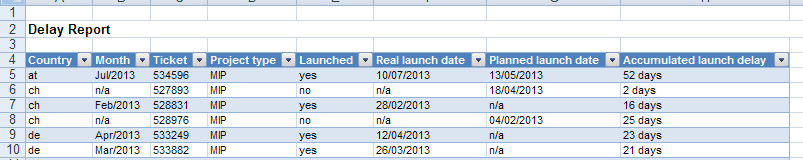
\includegraphics[width=1\textwidth]{./resources/report_delays.png}
   	\caption{Delays report}
   	\label{f_report_delays}
\end{figure}
\begin{figure}[ht!]
	\centering
   	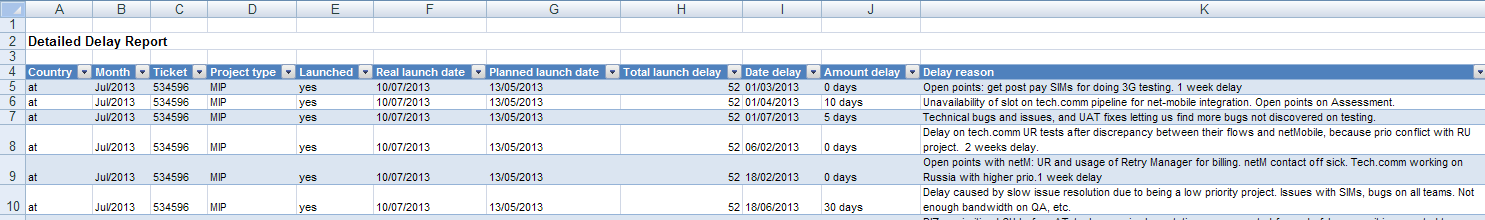
\includegraphics[width=1\textwidth]{./resources/report_delays_detail.png}
   	\caption{Detailed delays report}
   	\label{f_report_delays_detail}
\end{figure}
\begin{figure}[ht!]
	\centering
   	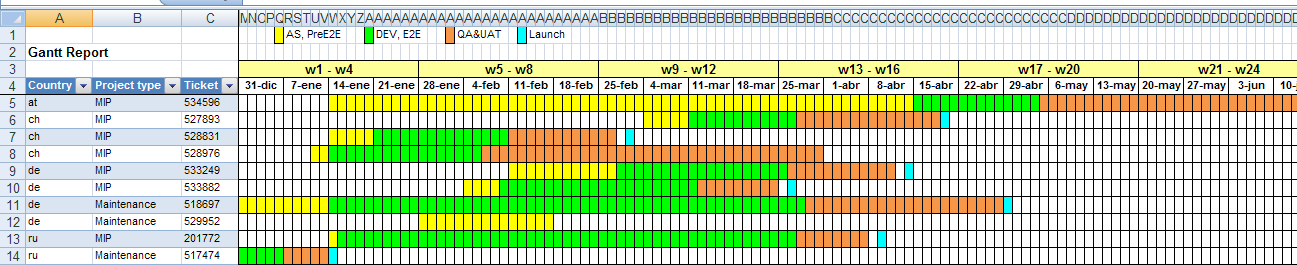
\includegraphics[width=1\textwidth]{./resources/report_gantt.png}
   	\caption{Gantt report}
   	\label{f_report_gantt}
\end{figure}
\begin{figure}[ht!]
	\centering
   	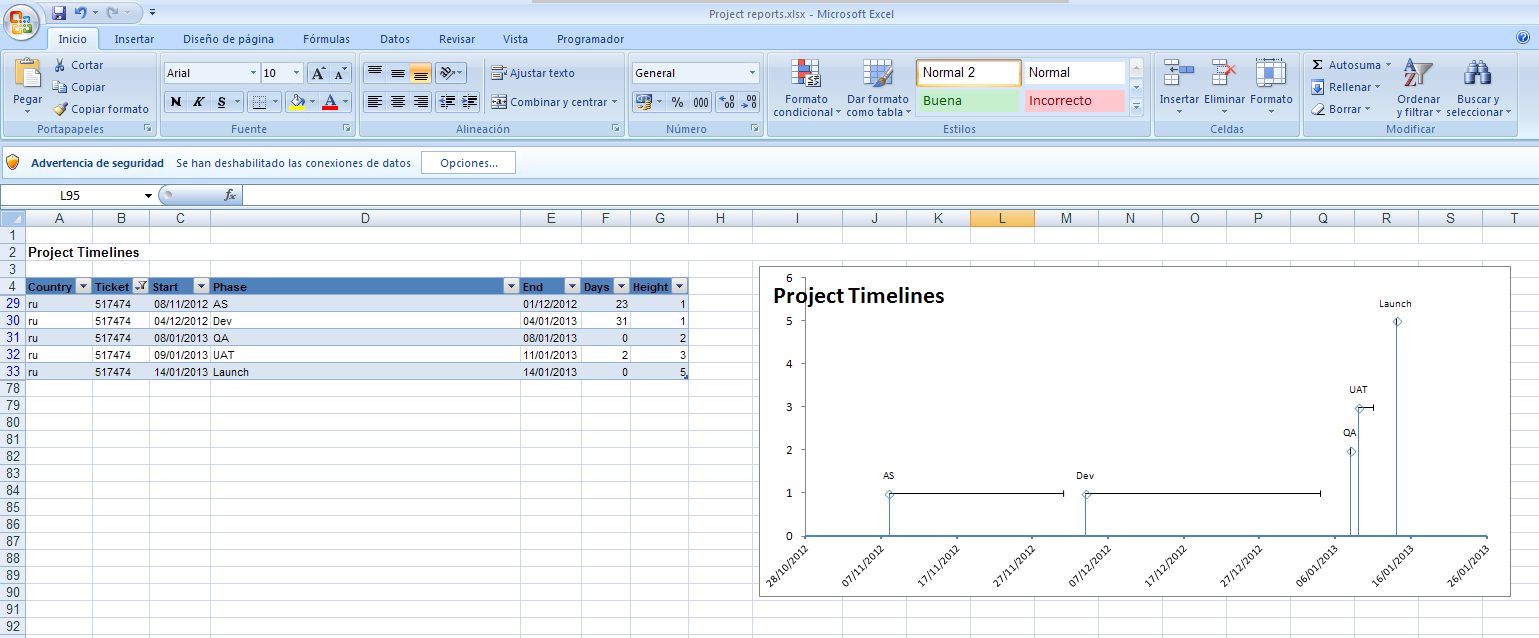
\includegraphics[width=1\textwidth]{./resources/report_timelines.png}
   	\caption{Timelines report}
   	\label{f_report_timelines}
\end{figure}
\begin{figure}[ht!]
	\centering
   	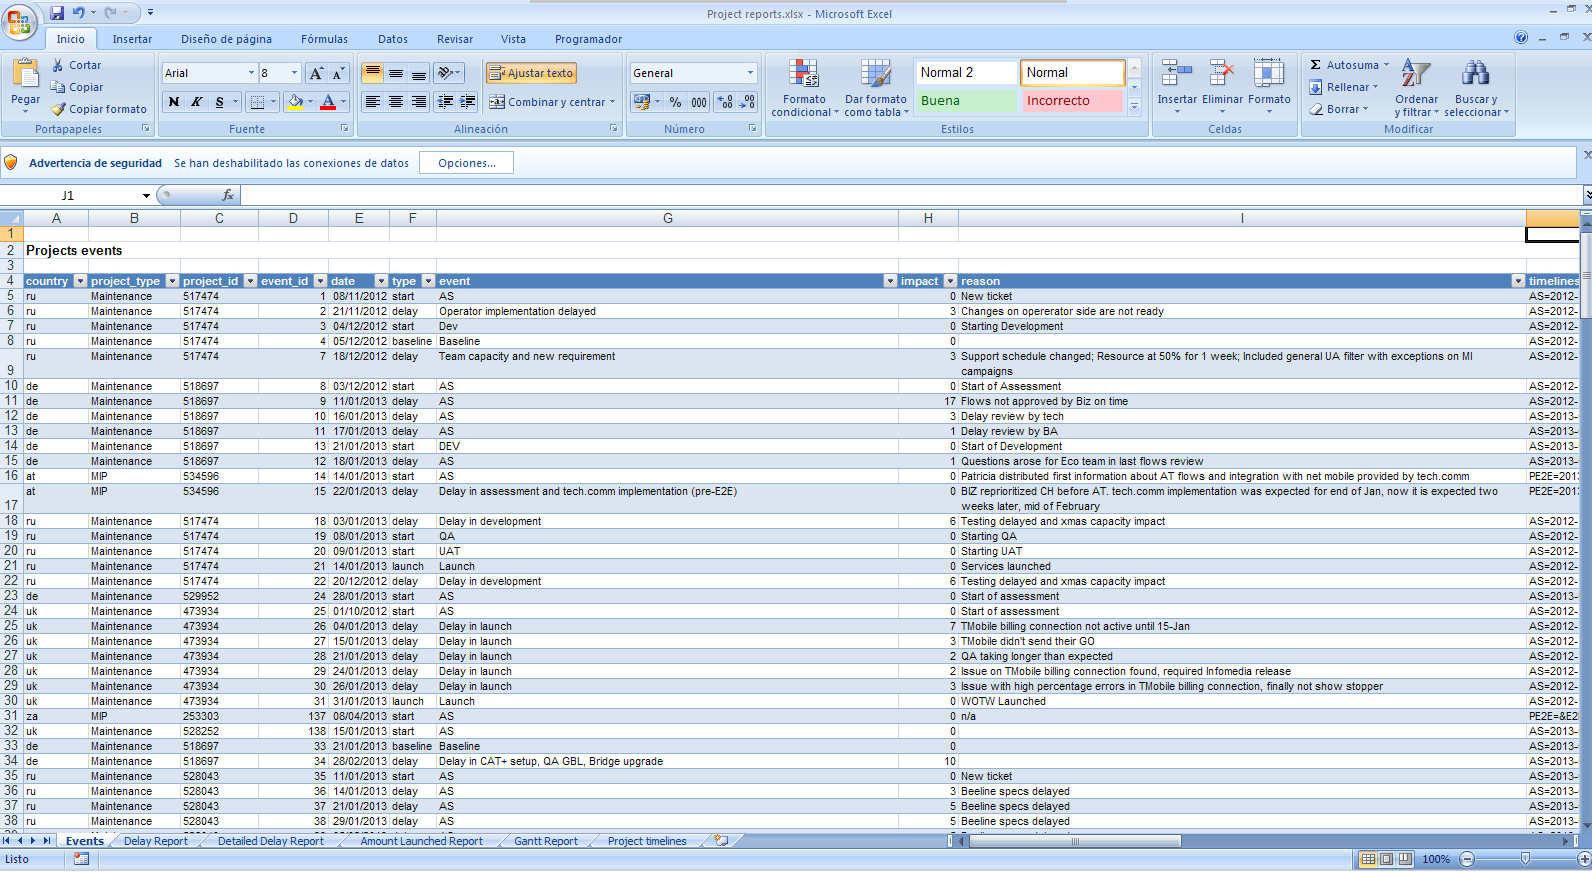
\includegraphics[width=1\textwidth]{./resources/report_events.png}
   	\caption{Events report}
   	\label{f_report_events}
\end{figure}

Each of those reports has defined one or more than one table's view that execute
the required data calculations and format the output in a Excel friendly way, so
the spreadsheet just need to show it and doesn't require any customization. 

This data and format coupling on the views definition was done on purpose,
in order to be flexible enough in the future in case was needed to define a
different viewer component, a part of the Excel, such as and HTML, or just
migrate it to a different platform. But, on both case the model could remain
untouched if the objective remained the same and only is needed to change the
view with a more powerful or friendly one. See and example on
\ref{f_report_launchesbymonth}.

\lstinputlisting[language=SQL,breaklines=true,caption=Launches
by month
view,label=f_report_launchesbymonth,frame=single,captionpos=b]{resources/report_launchesbymonth.sql}

In the other hand, decoupling it will need to be taken sooner or later if
we want to have a flexible and scalable tool, but this will be part of the
future work.

\section{The issue and what to improve}
As slightly tackled on previous sections, building a reporting tool based on
Excel was not the better solution, but it covered the main needs, even if we
faced issues like slowness, a single shared spreadsheet to be used by all
project managers, every report has a standalone database connection with the
possible impact on resources it could have and manual database insert per
each project's event.

All these points will be reviewed and covered on the next chapter. 

\chapter{New RESTful architecture}
After few time working with the spreadsheet linked with the database, and having
listed its downsides, I have started thinking about how to improve it without
affecting the main objective \ref{t_main_objective} but making it more
user friendly.

We already had listed the weaknesses and thinking on them, just came
up that the main change would be to replace completely the view (Excel), that
will solve all the issues, but will lose the power of the pivot table and
filters, but it could be managed in a second or third stage.

Now the question is: what could be the best replacement?

\section{Looking for a view replacement}
I wanted to have a very light view and user friendly, something that
provides directly the information to the user, a dashboard where the user could
see in one single view all the information he wants to see.

Nowadays, there are good examples of dynamic data dashboards done with the
latest online technologies like
Graphite\footnote{\url{http://graphite.wikidot.com/}},
Dashing\footnote{\url{http://shopify.github.io/dashing/}} or even using Google
Charts that could provide a good
dashboard\footnote{\url{https://developers.google.com/chart/}}.  Why online,
because today everything is connected and you can interact with almost everything, and
why not with the status of a project? Also, if you are not connected you are
not cool and very unuseful, and I wanted to have a useful tool, and why not,
also have a cool tool!

On top of that, objective is challenging, so better to go for a Lean
approach
\footnote{\url{http://en.wikipedia.org/wiki/Lean\_software\_development}} and
deliver small pices with the enough functionality even if they are not covering the final objective. So, following this approach the first objective was to have
a simple view of what we are managing here, projects and dates. So using Google
Charts we have enough to start and close the first phase. Also using a very
plain HTML and CSS code to provide the simplest functionality to enter the
required data.

\section{Looking for a REST server}
Once we have clear what is the view, we can start thinking about what could be
the best option to process the data we are going to use on the view.

We already knew that the architecture was going to be a server-client one and
mostly using REST approach in order to minimize the coupling between the
components, but there are many frameworks and web servers that provide this
functionality and further more, so what could fit better on our model?

One think I had very clear is I was looking for a Java implementation, why?
Because it provide a big amount of possible frameworks and technologies to
use or plug in and also maybe because I am more familiar and confident
with it.

Within the big umbrella of available Java servers
\footnote{\url{http://en.wikipedia.org/wiki/Comparison\_of\_application\_servers\#Java}},
I found Jersey \footnote{\url{https://jersey.java.net/}}, a RESTful web server
implemented in Java, that covers all my needs. A frameworks available just to
develop RESTful components, just what I was looking for.

A part of the REST framework, I found too Grizzly
\footnote{\url{https://grizzly.java.net/}} as a Server application, that will
provide to my tool a better scalable future in case I need it taking
advantage of Java NIO\footnote{\url{https://www.jcp.org/en/jsr/detail?id=51}}.

Now that seems that we have everything in place, we can start to open Eclipse
and start typing the code that will replace the spreadsheet. But this will be
part of the migration plan described on the following chapter.

\chapter{Migration plan}
Do not forget that the target is to deliver a \emph{simple} tool that replace
current Excel, so the migration will start developing the minimum code in order
to add, update and delete project's events and also provides the same
information that currently to the view in order to show it.

Considering also that we are not familiar with Grizzly and Jersey, first thing
will be to deploy a very simple server and REST application, using the examples,
in order to understand the logic and the process. You can find all the
information on the project webpage as well the tutorials and the examples that
will drive and help you on few typical scenarios.

Once we are confident with the framework we started to migrate the code and
defining the REST methods.

\section{REST methods}
Main methods will be defined under
\texttt{net.nuevegen.dashboard.reports.Reports} class where it will handle
the definition and implementation of all reports available, and covering as well
the addition and remove event's actions. 

So just in order to exemplify how easy is the implementation of a REST method
see getTimelinesByProjects method that fits with the implementation required to
show \ref{f_report_timelines}.

\begin{lstlisting}[language=Java,breaklines=true,caption=Reports.getTimelinesByProjects(),label=f_migration_gettimelines,frame=single,captionpos=b,numbers=left,
] @GET
@Consumes(MediaType.APPLICATION_JSON)
@Produces(MediaType.APPLICATION_JSON)
@Path("timelines{id : (/[a-zA-Z0-9]+)?}")
public Response getTimelinesByProject(@PathParam("id") String id) {
	Response response = null;
	List<Timeline> timelines = new LinkedList<Timeline>(); 

	...
	
	String query = "SELECT * FROM ukint_project_timelines_reports WHERE 1 ";

	if (id != null && id.trim().length()>0){
		query += "AND ticket='"+ id.replace("/", "") +"'";
	}
	
	st = Dashboard.getConnection(false).prepareStatement(query);
	rs = st.executeQuery();
	
	...
	
	GenericEntity<List<Timeline>> entity = new GenericEntity<List<Timeline>>(timelines) {};
	response = Response.ok(entity).build();
	
	...
	
	return response;
}
\end{lstlisting}

As you can see the annotation defined on this function allows us to specify what
kind of HTTP method will listen (GET, POST, PUT, etc..) and the uri under which
it will be executed, also the type of the data received (Consumes) and as well
the type of data returned (Produces). Those annotation makes the developer's
live more stresfuless because the final code required is encapsulated on the
annotations and will be injected as soon as it is required.

Finally, the code \texttt{Response.ok(entity)} on line 22 allows us to rewrite
the standard HTTP response and send to the client a specific HTTP/200 code with the
list of entities read from the database.

\section{Implementing the view}

\chapter{Conclusions}

\chapter{Future work}
\begin{itemize}
	\item Refactor database connectivity using a proper JPA based framework.
  
	Implement a real database connection pool using one of the existing persistence
	frameworks that implements JPA\footnote{Java Persistence API:
	\url{http://www.oracle.com/technetwork/articles/javaee/jpa-137156.html}}.
	
	\item Remove data-format coupling returned to the client.
	\item Refactor client making it usable for the final user (requires assessment
	and evaluation of main actions to carry out by the user).
\end{itemize}

%\begin{appendices}
%\chapter{Table views reports}
%\lstinputlisting[language=SQL,breaklines=true]{resources/reports_views.sql}
%\end{appendices}
